% !TEX encoding = IsoLatin

% La riga soprastante serve per configurare gli editor TeXShop, TeXWorks
% e TeXstudio per gestire questo file con la codifica IsoLatin o Latin 1
% o ISO 8859-1.

% per commentare una riga mettere % al suo inizio
% per s-commentare una riga (ossia attivarla) togliere il % al suo inizio
%
\documentclass[pdfa% formato PDF/A, obbligatorio per l'archiviazione delle tesi di Polito
%,cucitura%lascia margine per la rilegatura
,twoside% per stampa fronte-retro (fortemente consigliato per tesi voluminose, opzionale per le altre)
,12pt% font pi? grande (12pt) rispetto a quello normalmente usato (11pt)
]{toptesi}
%
\PassOptionsToPackage{dvipsnames}{xcolor}
\usepackage{url}
\usepackage{breakurl}
\usepackage[breaklinks]{hyperref}
\def\UrlBreaks{\do\/\do-}
\hypersetup{%
    pdfpagemode={UseOutlines},
    bookmarksopen,
    pdfstartview={FitH},
    colorlinks,
    linkcolor={blue},
    citecolor={red},
    urlcolor={blue}
  }
% \documentclass[11pt,twoside,oldstyle,autoretitolo,classica,greek]{toptesi}
% \usepackage[or]{teubner}
%%%%%%%%%%%%%%%%%%%%%%%%%%%%%%%%%%%%%%%%%%%%%%%%%%%%
%
% Esempio di composizione di tesi di laurea.
%
% Questo esempio e' stato preparato inizialmente 13-marzo-1989
% e poi e' stato modificato via via che TOPtesi andava
% arricchendosi di altre possibilita'.
%
% Nel seguito laurea "quinquennale" sta anche per "specialistica" o "magistrale"

% Cambiare encoding a piacere; oppure non caricare nessun encoding se si usano
% solo caratteri a 7 bit (ASCII) nei file d'entrata.
%
\usepackage[latin1]{inputenc}% IMPORTANTE! usare codifica ISO-8859-1 per le lettere accentate
% \usepackage[outputdir=out,cache=false]{minted}

% !TEX encoding = IsoLatin

% per inserire uno spazio "fantasma" nella definizione di un'abbreviazione
\usepackage{xspace}

% per inserire un DOI senza problemi coi caratteri "strani" ivi presenti
\usepackage{doi}
\renewcommand{\doitext}{DOI }% originally was "doi:"

% per inserire correttamente le unit� di misura SI (incluse quelle binarie)
\usepackage[binary-units]{siunitx}
% se si desidera usare / invece che la potenza -1 per indicare "al secondo"
\sisetup{per-mode=symbol}

% per inserire codice di programmazione complesso
\usepackage{listings}% per inserire codice di programmazione complesso
\lstset{
basicstyle=\ttfamily,
columns=fullflexible,
xleftmargin=3ex,
breaklines,
breakatwhitespace,
escapechar=`
}

% modify some page parameters
\setlength{\parskip}{\medskipamount}

% riga orizzontale
\newcommand{\HRule}{\rule{\linewidth}{0.2mm}}
% esempio di creazione di semplici abbreviazioni
\newcommand{\ltx}{\LaTeX\xspace}
\newcommand{\txw}{TeXworks\xspace}
\newcommand{\mik}{MikTex\xspace}
\newcommand{\html}{HTML\xspace}
\newcommand{\xhtml}{XHTML\xspace}

% esempio di creazione di un'abbreviazione con un parametro (il cui uso � indicato da #1)
\newcommand{\cmd}[1]{\texttt{#1}\xspace}
% per citare un RFC, es. \rfc{822}
\newcommand{\rfc}[1]{RFC-#1\xspace}
% per citare un file (es. \file{autoexec.bat}) o una URI fittizia (es. \file{http://www.lioy.it/})
% per le URI vere usare \url o \href
\newcommand{\file}[1]{\texttt{#1}\xspace}
% per inserire codice di esempio in-line
\newcommand{\code}[1]{\lstinline|#1|}
% importante per i pathname Windows perch� non si pu� usare \ essendo un carattere riservato di Latex
\newcommand{\bs}{\textbackslash}
% definizione di un termine: formattazione ed inserimento nell'indice
\newcommand{\tdef}[1]{\textit{#1}\index{#1}}
% meta-termine, usato tipicamente nelle definizioni dei tag
\newcommand{\meta}[1]{\textit{#1}}
% abbreviazioni in inglese
\newcommand{\ie}{i.e.\xspace}
\newcommand{\eg}{e.g.\xspace}
\usepackage{cryptocode}
\usepackage{svg}
\usepackage{plantuml}
% modificare il path di inkscape nel caso di errori
\setsvg{inkscape={"C:/Program Files/Inkscape/bin/inkscape.com"}}
\svgpath{{chapters/images}}

\usepackage{enumitem}
\usepackage{booktabs}
\usepackage{fontawesome}
\usepackage{multicol}
\usepackage{xcolor}
\usepackage{tcolorbox}
\usepackage{placeins}
\usepackage{float}
\newtcolorbox{mybox}{colback=red!5!white,colframe=red!75!black}
\lstdefinestyle{json}{
  string=[s]{"}{"},
  stringstyle=\color{blue},
  comment=[l]{:},
  commentstyle=\color{black},
}
\lstdefinestyle{DOS}{
  backgroundcolor=\color{black},
  basicstyle=\color{white}\ttfamily
}

\makeatletter
\def\lst@visiblespace{\lst@ttfamily{\phantom{\char32}}{\phantom{\textvisiblespace}}}
\begin{document}
\selectlanguage{english}


\ateneo{Politecnico di Torino}

%%% scegliere la propria facolt? (solo PRIMA dell'AA 2012-2013)
%
%\facolta[III]{Ingegneria dell'Informazione}
%\facolta[IV]{Organizzazione d'Impresa\\e Ingegneria Gestionale}
%\Materia{Remote sensing}% uso sconsigliato

%\monografia{Gestione informatizzata di un magazzino ricambi}% per la laurea triennale
\titolo{Self-Sovereign-Identity as a Service}% per la laurea quinquennale e il dottorato
\sottotitolo{Trusted computation offloading for IoT constrained devices}% NON obbligatorio, per la laurea quinquennale e il dottorato

%%% scegliere il proprio corso
%
%\corsodilaurea{Ingegneria dell'Organizzazione d'Impresa}% per la laurea di primo e secondo livello
%\corsodilaurea{Ingegneria Logistica e della Produzione}% per la laurea di primo e secondo livello
%\corsodilaurea{Ingegneria Gestionale}% per la laurea di primo e secondo livello
\corsodilaurea{Computer Engineering}% per la laurea di primo e secondo livello
%\corsodidottorato{Meccanica}% per il dottorato

\candidato{Luca \textsc{Giorgino}}% per tutti i percorsi
%\secondocandidato{Evangelista \textsc{Torricelli}}% per la laurea magistrale solamente
%\direttore{prof. Albert Einstein}% per il dottorato
%\coordinatore{prof. Albert Einstein}% per il dottorato
\relatore{prof.\ Antonio Lioy}% per la laurea e il dottorato
%\secondorelatore{dipl.~ing.~Werner von Braun}% per la laurea magistrale
%\terzorelatore{{\tabular{@{}l}dott.\ Neil Armstrong\\prof. Maria Rossi\endtabular}}% per la laurea magistrale
%\tutore{ing.~Karl Von Braun}% per il dottorato
%\tutoreaziendale{PhD.\ ing.\ Andrea Vesco} % solo per la laurea di secondo livello con tesi svolta in azienda
\tutoreaziendale{Andrea Vesco, Ph.D.\\Alberto Carelli, Ph.D.} % solo per la laurea di secondo livello con tesi svolta in azienda
% \NomeTutoreAziendale{Supervisore aziendale\\LINKS FOUNDATION}
%\sedutadilaurea{Ottobre 2022}% per la laurea quinquennale
%\esamedidottorato{Novembre 1610}% per il dottorato
%\sedutadilaurea{\textsc{Ottobre} 2022}% per la laurea triennale
\sedutadilaurea{\textsc{Academic~year} 2021-2022}% per la laurea magistrale
%\annoaccademico{1615-1616}% solo con l'opzione classica
%\annoaccademico{2006-2007}% idem
%\ciclodidottorato{XV}% per il dottorato
\logosede{other/logopolito}
%
%\chapterbib %solo per vedere che cosa succede; e' preferibile comporre una sola bibliografia
%\AdvisorName{Supervisors}
%\newtheorem{osservazione}{Osservazione}% Standard LaTeX

%\usepackage[a-1b]{pdfx}
%\hypersetup{%
%    pdfpagemode={UseOutlines},
%    bookmarksopen,
%    pdfstartview={FitH},
%    colorlinks,
%    linkcolor={blue},
%    citecolor={green},
%    urlcolor={blue}
%  }

%
% per numerare e far comparire nell'indice anche le sezioni di quarto livello
% SCONSIGLIATO! da usarsi solo in caso di estrema necessit?
%\setcounter{secnumdepth}{4}% section-numbering-depth
%\setcounter{tocdepth}{4}% TOC-numbering-depth (TOC=Table-Of-Content)

%\setbindingcorrection{3mm}

\errorcontextlines=9

\iflanguage{english}{
  %\retrofrontespizio{This work is subject to the Creative Commons Licence}
  \DottoratoIn{PhD Course in\space}
  \CorsoDiLaureaIn{Master degree course in\space}
  \NomeMonografia{Bachelor Degree Final Work}
  \TesiDiLaurea{Master Degree Thesis}
  \NomeDissertazione{PhD Dissertation}
  \InName{in}
  \CandidateName{Candidate}
  \AdvisorName{Supervisor}
  \TutorName{Tutor}
  \NomeTutoreAziendale{Tutors\\LINKS FOUNDATION}
  \CycleName{cycle}
  \NomePrimoTomo{First volume}
  \NomeSecondoTomo{Second Volume}
  \NomeTerzoTomo{Third Volume}
  \NomeQuartoTomo{Fourth Volume}
}{}

\frontespizio
\paginavuota
\newpage
%per sfruttare meglio lo spazio nella pagina
\advance\voffset -5mm
\advance\textheight 30mm

% opzionale, solo se si vuole dedicare la tesi a delle persone care
% \begin{dedica}
% To my parents
% \end{dedica}

\sommario

% Digital identity makes IoT objects unique and distinguishes them from each other. Self-Sovereign Identity aims to provide a digital identity that is both verified and verifiable to IoT objects while building a digital ecosystem for secure interactions between heterogeneous objects. However, in many real-world use cases, IoT devices are constrained and cannot run natively a full Self-Sovereign Identity stack implementation. For this reason, an edge device has been designed with the capability of supporting a constrained device to create and manage its own self-sovereign identity and it has been developed using Keystone, an open-source framework for building Trusted Execution Environments, providing trust in the system that handles offloaded operations. Such a solution has the advantage to increase the number of devices that can interact in a secure digital ecosystem of this kind and defines a new paradigm called Self-Sovereign Identity as a Service. 

Digital identity makes IoT objects unique and distinguishes them from each other. Self-Sovereign Identity (SSI) aims to provide a digital identity that is both verified and verifiable to IoT objects while building a digital ecosystem for secure interactions between heterogeneous objects. However, in many real-world use cases, IoT devices cannot run natively a full self-sovereign identity stack implementation, due to hardware and software constraints. For this reason, an edge device has been designed with the capability of securely aiding constrained devices to create and manage their own identity according to the SSI paradigm. The software has been developed using Keystone, an open-source framework for building Trusted Execution Environments, for establishing a trusted communication channel between the IoT device and the edge device that handles offloaded operations. By defining a new paradigm called Self-Sovereign Identity as a Service, constrained devices can exploit the full SSI stack on demand. Such a solution has the advantage to increase the number of devices that can interact in a secure digital ecosystem of this kind by shifting the computational operations onto more powerful edge devices. 

\ringraziamenti

I would like to thank Professor Antonio Lioy for his supervision. I sincerely thank Ing. Andrea Vesco, Ing. Alberto Carelli and Ing. Davide Margaria, the Cybersecurity team of LINKS Foundation, for their precious advice, continuous support and provided knowledge during the realization of this work. 

I thank my family, who sustained me throughout my university career. In particular, I thank my father and my mother. Without them, this day would not have been possible. Finally, I would like to extend a special thanks to Elisabetta, who has always shown me her encouragement and love during these years of study.
%% inserire sempre nella tesi per la laurea di I livello, perch? il nome dei tutori non ? indicato sul frontespizio.
%Il lavoro descritto in questa monografia ? stato svolto sotto la supervisione
%del Prof. Antonio Lioy (tutore accademico)% inserire sempre il nome del tutore accademico
% e dell'Ing. Mario Rossi (tutore aziendale)% inserire solo se la monografia ? relativa ad un tirocinio.
%.

%\tablespagetrue % normalmente questa riga non serve ed e' commentata
%\figurespagetrue % normalmente questa riga non serve ed e' commentata

\indici

\mainmatter

\chapter{Introduction}
%!TEX encoding = IsoLatin
%!TEX main = ../../main.tex

The concept of digital identity has been evolving in the last decades. Digital identity is the expression and storage of one's identity in digital form, which is a set of claims, i.e., assertions of some truths, made about a person or a thing, also named subject. Despite this, only in recent years privacy, control and ownership over digital identity and personal data are being increasingly recognized as relevant factors by individuals \cite{TheLawsOfIdentity}. 
Since the advent of the Internet, digital identity models have gone through several stages, from centralized identity to federated identity, becoming more user-centric over time until we reach the point where we are talking about Self-Sovereign Identity \cite{ThePathToSSI}.
In the Internet's early days, digital identity issuers and authenticators were centralized authorities. Unfortunately, giving centralized authorities control over a user's digital identity has several drawbacks, a single authority can deny a user's identity or even confirm a false one, so the user has no control over his own identity. Self-sovereign identity is the next development of digital identity and the main idea is that the user must be at the centre of identity management \cite{ThePathToSSI}.


The Internet of Things increasingly involves the collection, processing and transmission of a wide variety of data to services and other devices \cite{wilson2018digital}. Reasonably obvious privacy risks arise from IoT-connected devices when they exchange identifiable information, as this can reveal the activities and behaviours of device users and subtle risks arise when a considerable amount of data is available for analysis and linkage to additional data sets, since user identification or re-identification may happen as a result \cite{wilson2018digital}. For building a digital realm where heterogeneous objects and people interact in a secure manner digital identity, such as self-sovereign identity, could be a solution, allowing IoT devices to be unique and distinguishable from one another.


In this document, self-sovereign identity is introduced, as well as keystone enclave, an open-source framework for trusted execution environments based on hardware enclaves. Then is presented the solution, which has been designed to support a constrained device to create and manage its own digital identity. 

% contesto
% problema
% soluzione

% The topics are organized as follows:
% \begin{itemize}
%     \item Chapter \ref{chap:1} 
%     \item Chapter \ref{chap:2} 
%     \item Chapter \ref{chap:3}
%     \item Chapter \ref{chap:4}
%     \item Chapter \ref{chap:5}
% \end{itemize}


\chapter{Self-Sovereign Identity}
%!TEX encoding = IsoLatin
%!TEX main = ../../main.tex

%\section{Self-Sovereign-Identity}
Self-Sovereign Identity (SSI) \cite{tobin2016inevitable} is a new model for digital identity. In the SSI ecosystem, a user can fully control his own identity and use it between any service. SSI is different from today's digital identities: it is anchored to distributed ledgers so is not controlled by any centralized services.
One SSI innovation is the design and development of a common set of specifications: 
Decentralized Identifiers (DIDs) \cite{didW3C} and Verifiable Credentials (VCs) \cite{vcW3C}. By doing this, user identity can be anchored to different distributed ledgers, but it will also be defined in the same standard way.

\section{Decentralized Identifiers}  
DIDs \cite{didW3C} are identifiers referring to any subject determined by the controller of the DID.
A DID's controller can demonstrate control over it thanks to the design without requesting permission from any other party allowing a verifiable, decentralized digital identity, that will be independent of identity providers, and certification authorities.

\subsection*{Overview}

In detail a DID is a type of URI \cite{berners2005uniform} scheme that links a DID subject with a DID document allowing trustable interactions associated with that subject. The subject of a DID is the entity identified by the DID and can be a person, a group or an organization. Typically the DID subject is also the controller, but a DID can have more than one. 

Specifically, a DID is a simple text string, as shown in the figure \ref{didExample}, consisting of three parts: 
\begin{itemize}
    \item the DID URI scheme identifier
    \item the identifier for the DID method
    \item the DID method-specific identifier
\end{itemize}

\begin{figure}[h!]
    \centering
    \includesvg[inkscapelatex=false, scale=0.70]{./chapters/images/parts-of-a-did.svg}
    \caption{A simple example of a DID \cite{didW3C}.}
    \label{didExample}
\end{figure}

A DID resolves to a DID document, a DID document contains information about a DID subject and cryptographic material that will be used to prove control of that DID. DID documents can be represented in JSON \cite{json-rfc3986} or JSON-LD \cite{json-ld} format, as can be seen in the figure \ref{didDocExample}. Only the controller of the DID has the right to make changes to the related DID document. 

DIDs are generally stored in some underlying system or network for the resolution to DID documents. A verifiable data registry is a system that enables the recording of DIDs and the return of the data required to produce DID documents. Distributed ledgers, decentralized file systems, all types of databases, peer-to-peer networks, and other trusted data storage methods are some examples. The operations to create, resolve, update, and deactivate a DID and the related DID document are defined by DID methods and their specifications, which are generally coupled with a distinct verifiable data registry \cite{didW3C}. 
A DID URL expands the syntax of a DID with other standard components of URI such as path, query, and fragment to find a specific resource, such as a cryptographic public key in a DID document or a resource outside the DID document. \\

% \begin{lstlisting}[caption={Example of a simple DID document from \cite{didW3C}.},captionpos=b,style=json, label={didDocExample},frame=single]
% {
%     "@context": [
%         "https://www.w3.org/ns/did/v1",
%         "https://w3id.org/security/suites/ed25519-2020/v1"
%     ]
%     "id": "did:example:123456789abcdefghi",
%     "authentication": [{

%         "id": "did:example:123456789abcdefghi#keys-1",
%         "type": "Ed25519VerificationKey2020",
%         "controller": "did:example:123456789abcdefghi",
%         "publicKeyMultibase": "zH3C2AVvLMv6gmMNam3uVAjZpfkcJCwDwnZn6z3wXmqPV"
%     }]
% }
% \end{lstlisting}

\begin{figure}[h!]
\begin{lstlisting}[style=json,frame=single]
{
    "@context": [
        "https://www.w3.org/ns/did/v1",
        "https://w3id.org/security/suites/ed25519-2020/v1"
    ]
    "id": "did:example:123456789abcdefghi",
    "authentication": [{

        "id": "did:example:123456789abcdefghi#keys-1",
        "type": "Ed25519VerificationKey2020",
        "controller": "did:example:123456789abcdefghi",
        "publicKeyMultibase": "zH3C2AVvLMv6gmMNam3uVAjZpfkcJCwDwnZn6z3wXmqPV"
    }]
}
\end{lstlisting}
\caption{Example of a simple DID document from \cite{didW3C}. \label{didDocExample}}
\end{figure}

\begin{figure}[h!]
    \centering
    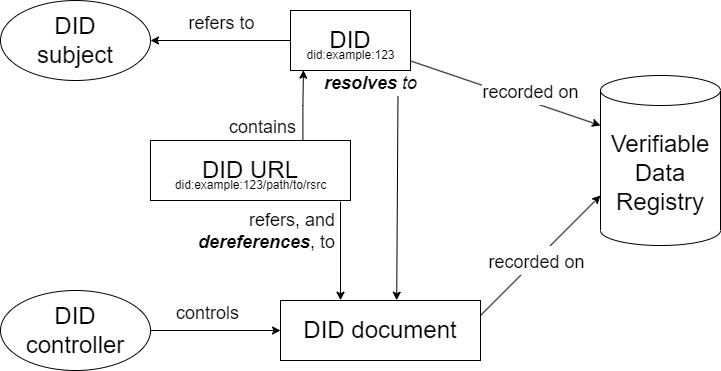
\includegraphics[width=10cm]{./chapters/images/did-overview.png}
    \caption{DID architecture overview and relationships between components \cite{didW3C}.}
    \label{didOverview}
\end{figure}

\section{Verifiable Credentials}
Verifiable Credential \cite{vcW3C} provides a standard method to express credentials on the internet in a way that is cryptographically safe, privacy-respecting, and machine-verifiable.
In our daily lives a credential could consist of:
\begin{itemize}
    \item information related to identifying the subject of the credential (for example, a photo, name, or identification number)
    \item information related to the issuing authority (for example, a city government or a university)
    \item information related to the type of credential this is (for example, a passport or a driving license)
    \item information related to specific attributes or properties being asserted by the issuing authority about the subject (for example, nationality, the classes of vehicle entitled to drive, or date of birth)
    \item information related to constraints on the credential (such as expiration date, or terms of use). 
\end{itemize}

In verifiable credentials, the inclusion of digital signatures makes them more trustworthy and more tamper-evident against physical credentials allowing third-party verified machine-readable personal information usable on the Web for receiving services and benefits as in the physical world \cite{vcW3C}.

\subsection*{Overview}

Distinct actors can be identified in the verifiable credentials ecosystem, which defines the roles and the relationships between them. The separation of roles allows the standardization of interfaces and protocols. In detail the existing entities that determine the \textit{trust triangle} \cite{trustOverIP} are: 

\begin{itemize}
    \item \textit{holder}: his role is to request, possess or use verifiable credentials. Example holders include students, employees, and customers.
    \item \textit{issuer}: his role is to create a verifiable credential and provide that to a holder by asserting claims about one or more subjects. For example, an issuer is a government. 
    \item \textit{verifier}: his role is to process verifiable credentials provided by holders. Example verifiers are whoever provides a service. 
\end{itemize}

\begin{figure}[h!]
    \centering
    \includesvg[inkscapelatex=false, scale=0.70]{./chapters/images/vc-ecosystem.svg}
    \caption{The roles and information flows of Verifiable Credential \cite{vcW3C}.}
    \label{vcEcosystem}
\end{figure}

To use verifiable credentials a holder has to generate verifiable presentations by enclosing them and signing before presenting them to a verifier, by doing this a holder demonstrates the possession of the verifiable credential. The fact that a credential is verifiable by the verifier does not mean that the claims it contains are true. Another aspect that variable credentials enhance is privacy. The usage of machine-readable credentials allows malicious actors to collect and correlate data, compromising holders' privacy. Variable credentials specification draft how to deal with these issues, by using privacy-enhancing technologies, such as \textit{zero-knowledge proof} \cite{zkp-survey}. 

\begin{figure}[h!]
    \centering
    \includesvg[inkscapelatex=false, scale=0.45]{./chapters/images/credential.svg} 
    \hfil
    \includesvg[inkscapelatex=false, scale=0.45]{./chapters/images/presentation.svg}
    \caption{Basic components of a verifiable credential and a verifiable presentation \cite{vcW3C}.}
    \label{vc-vp-topview}
\end{figure}

Verifiable credentials and verifiable presentations can be represented in JSON \cite{json-rfc3986} or JSON-LD \cite{json-ld} format as can be seen in figures \ref{vcExample} and \ref{vpExample}. \\

\begin{figure}[h!]
\begin{lstlisting}[style=json, breaklines=true,frame=single]
{
    "@context": [
        "https://www.w3.org/2018/credentials/v1",
        "https://www.w3.org/2018/credentials/examples/v1"
    ],
    "id": "http://example.edu/credentials/1872",
    "type": ["VerifiableCredential", "AlumniCredential"],
    "issuer": "https://example.edu/issuers/565049",
    "issuanceDate": "2010-01-01T19:23:24Z",
    "credentialSubject": {
        "id": "did:example:ebfeb1f712ebc6f1c276e12ec21",
        "alumniOf": {
            "id": "did:example:c276e12ec21ebfeb1f712ebc6f1",
            "name": [{
                "value": "Example University",
                "lang": "en"
            }]
        }
    },    
    "proof": {
        "type": "RsaSignature2018",
        "created": "2017-06-18T21:19:10Z",
        "proofPurpose": "assertionMethod",
        "verificationMethod": "https://example.edu/issuers/565049#key-1",
        "proofValue": "eyJhbGciOiJSUzI1NiIsImI2NCI6ZmFsc2UsI..."
        }
}
\end{lstlisting}
\caption{A simple example of a verifiable credential \cite{vcW3C}. \label{vcExample}}
\end{figure}

% \begin{lstlisting}[caption={A simple example of a verifiable presentation \cite{vcW3C}.},captionpos=b,style=json, label={vpExample},breaklines=true,frame=single]
%     {
%         "@context": [
%           "https://www.w3.org/2018/credentials/v1",
%           "https://www.w3.org/2018/credentials/examples/v1"
%         ],
%         "type": "VerifiablePresentation",
%         "verifiableCredential": [{
%             ...
%         }],
%         "proof": {
%           "type": "RsaSignature2018",
%           "created": "2018-09-14T21:19:10Z",
%           "proofPurpose": "authentication",
%           "verificationMethod": "did:example:ebfeb1f712ebc6f1c276e12ec21#keys-1",
%           "challenge": "1f44d55f-f161-4938-a659-f8026467f126",
%           "domain": "4jt78h47fh47",
%           "proofValue": "Qy72IFLN25DYuNzVBAh4vGHSrQyHUGlc..."
%         }
%       }   
% \end{lstlisting}


\begin{figure}[h!]
\begin{lstlisting}[style=json, breaklines=true,frame=single]
{
    "@context": [
        "https://www.w3.org/2018/credentials/v1",
        "https://www.w3.org/2018/credentials/examples/v1"
    ],
    "type": "VerifiablePresentation",
    "verifiableCredential": [{
        ...
    }],
    "proof": {
        "type": "RsaSignature2018",
        "created": "2018-09-14T21:19:10Z",
        "proofPurpose": "authentication",
        "verificationMethod": "did:example:ebfeb1f712ebc6f1c276e12ec21#keys-1",
        "challenge": "1f44d55f-f161-4938-a659-f8026467f126",
        "domain": "4jt78h47fh47",
        "proofValue": "Qy72IFLN25DYuNzVBAh4vGHSrQyHUGlc..."
    }
}   
\end{lstlisting}
\caption{A simple example of a verifiable presentation \cite{vcW3C}. \label{vpExample}}
\end{figure}
\FloatBarrier   
\section{Distributed Ledgers Technologies}

Distributed Ledger Technology (DLT)  is a new paradigm for collecting and sharing information between people. A distributed ledger is a database that is spread across several nodes or computing devices. An exact copy of the ledger is replicated and stored on each node. The revolutionary aspect of distributed ledger technology is that no single administrator or central authority is responsible for maintaining the ledger. Each network's participant node keeps its state updated by constructing and recording updates to the ledger independently. The nodes then vote on these adjustments to ensure that the majority agrees with the conclusion reached. This voting and agreement on the state of the ledger is called consensus and is conducted automatically via a consensus algorithm \cite{dlt-intro-1}. 
The following criteria can be used to categorize DLTs: data structures, consensus algorithms, permissions, mining accessibility and so on. The main data structure types are blockchains and Directed Acyclic Graphs (DAGs). Although blockchains are the most popular and well-known DLT type,  DLTs based on Directed Acyclic Graph (DAG) data structures are becoming more popular because they reduce transaction data size and transaction fees, and increase transaction speeds \cite{dlt-intro-2}.

An Example of DAG DLT is the \textit{tangle} of IOTA \cite{popov2018tangle}, a cryptocurrency for the Internet-of-Things (IoT) industry.

\begin{figure}[h!]
    \centering
    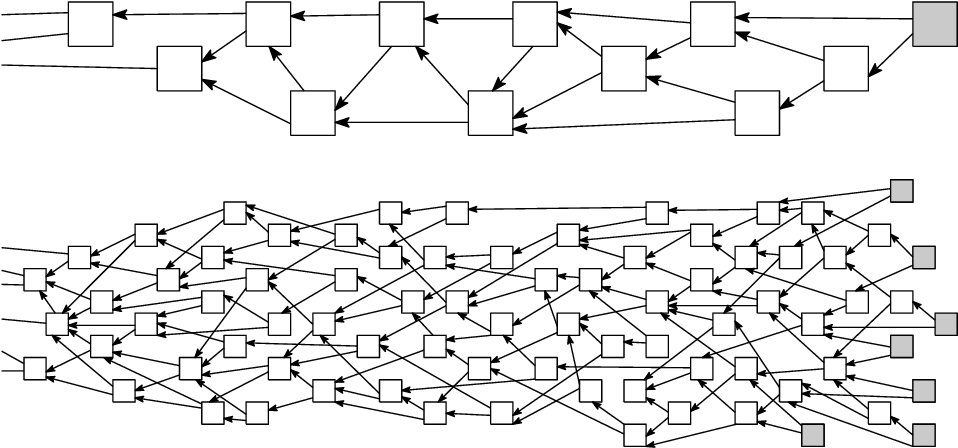
\includegraphics[width=10cm]{./chapters/images/tangle.png}
    \caption{Visualizations of the IOTA tangle \cite{popov2018tangle}.}
    \label{tangleFigure}
\end{figure}

%parlare di come e' immutabile una blockchain?
\chapter{Kestone Enclave}
%!TEX encoding = IsoLatin
%!TEX main = ../../main.tex

%\section{Keystone Enclave}
%todo modificare questa intro
Device manufacturers are now taking security concerns more seriously than they previously did as a result of the rise in the popularity of networked devices in recent years.
To adequately address these challenges, Trusted Execution Environments have been developed that define a way to ensure the integrity and confidentiality of sensitive data in the device that implements the specification \cite{IntroTEE}. Keystone \cite{lee2020keystone} is an open-source framework for creating RISC-V hardware-based Trusted Execution Environments that are adaptable for use on a variety of platforms. 

\section{Trusted Execution Environment}
A Trusted Execution Environment (TEE) is a safe area within a CPU. It runs in an isolated environment and in parallel with the operating system.
It ensures that the confidentiality and integrity of the code and data loaded in the TEE are preserved. 
Trusted applications running on TEE have access to the full capabilities of a device's main processor and memory, while hardware isolation shields these components from user-installed apps running in the main operating system. The various included trusted applications are protected from one another by software and cryptographic isolations within the TEE \cite{IntroTEE}.
The two most common TEE implementations at the moment are ARM TrustZone and Intel SGX. All these TEEs make design decisions based on either the target applications or threat models and these choices are fixed since they are strictly hardware related. They were not designed to have flexibility or extensibility for enclave developers. If the hardware changes or has a new feature, the enclave developer has to redesign the TEE.
All TEE platforms aim to reduce the enclave's Trusted computing Base, yet they have managed to achieve different degrees of success \cite{keysyone-blog-1}. The Trusted Computing Base (TCB) is a section of the system, it could include hardware, firmware and software, which is responsible for enforcing the security policy of the system \cite{tcb-def}. Additionally, closed-source hardware and microcode implementations make it impossible for a third party to evaluate the security of TEEs.

\subsection{Customizable Trusted Execution Environment}
Customizable TEE is the solution to these problems. It has been designed to be flexible, and configurable and to have a small TCB. It has been designed with clear abstractions and a modular programming model which simplifies for others to extend and add features to the TEE. A customizable TEE is Keystone \cite{lee2020keystone}. Three logical actors, such as the manufacturer (who makes the hardware), the platform provider (runs the hardware, such as a cloud provider), and the enclave developer (who writes software that runs in the enclaves), were identified by keystone developers as being a part of the customizable TEE ecosystem. In a customizable TEE, as opposed to a standard TEE, decisions made by all 3 actors together determine the security guarantees offered and the functionalities enabled \cite{keysyone-blog-1}. 
Keystone offers security primitives that can be joined together via the software framework rather than creating a single instance of TEE hardware. The TEE can be modified by the creator of the enclave and the platform provider to suit their threat models or platform configurations. The Keystone project offers a general and formally proven interface for a variety of devices to create an open standard for TEEs. 

\section{RISC-V Background}
RISC-V offers several advantages, apart from being open-source, security-oriented primitives have been added that provide efficient isolation, the most notable being Physical Memory Protection (PMP). RISC-V is an evolving and community-driven Instruction Set Architecture (ISA). Keystone can be designed and developed using standard features and the ever-growing world of RISC-V gives Keystone a wide variety of potential platforms and different deployment scenarios to which it can adapt to. \cite{keysyone-blog-2}

\subsection{RISC-V Privilieged ISA}
RISC-V \cite{risc-v-spec} has three software privilege levels (in increasing order of capability): user mode (U-mode), supervisor mode (S-mode), and machine mode (M-mode). Only one of the privilege modes can be active on the processor at once.
The active privilege level determines what the software can do while it is running. These are typical applications for each level of privilege:
\begin{itemize}
    \item U-mode: user processes 
    \item S-mode: kernel (including kernel modules and device drivers) or hypervisor
    \item M-mode: bootloader and firmware
\end{itemize}
When the processor is in the highest privilege mode, M-mode, it is in control of all physical resources and interrupts. As with microcode in Complex Instruction Set Computer (CISC) ISAs (such as x86), M-mode is not interruptible and not affected by the interference of lower modes. M-mode is used in Keystone for executing the TCB of the system, the \textit{security monitor} (SM).
\begin{figure}[h!]
    \centering
    \includesvg[inkscapelatex=false, scale=0.40]{./chapters/images/TEE-keystone-vs-x86.svg}
    \caption{Architecture differences between x86 and keystone}
    \label{keystone-vs-x86}
\end{figure}
The following are some advantages of utilizing an M-mode software as the TCB:
\begin{itemize}
    \item Programmability: unlike microcode for x86, in RISC-V M-mode software can be written using pre-existing toolchains and programming languages, such as C. 
    \item Agile Patching: since the TCB is purely software, bugs or vulnerabilities can be patched without updates, which are specific to a particular hardware 
    \item Verifiability: compared to hardware, the software is generally simpler to be formally verified.
\end{itemize}

\subsection{Physical Memory Protection}
Physical Memory Protection (PMP) is a strong standard primitive that enables M-mode to control the access to physical memory from lower privileges modes. Keystone requires PMP to implement memory isolation of enclaves.
Only software in M-mode can configure the PMP, which is controlled by a series of control and status registers (CSR) that limit physical memory access to the U-mode and S-mode. Depending on the platform design, PMP entries number can change. 
Since PMP exclusively works on physical addresses, S-mode can continue to support virtual addresses without affecting the security of the system. Even though each processor may implement PMP differently in hardware, the basic guarantees are part of the standard. PMP is used by Keystone Security Monitor to create memory isolation.

\section{Keystone components}
\label{keystone-components}
A Keystone-capable system is made up of different modules operating in various privilege modes as shown in figure \ref{keystoneComponents}.

\begin{figure}[h!]
    \centering
    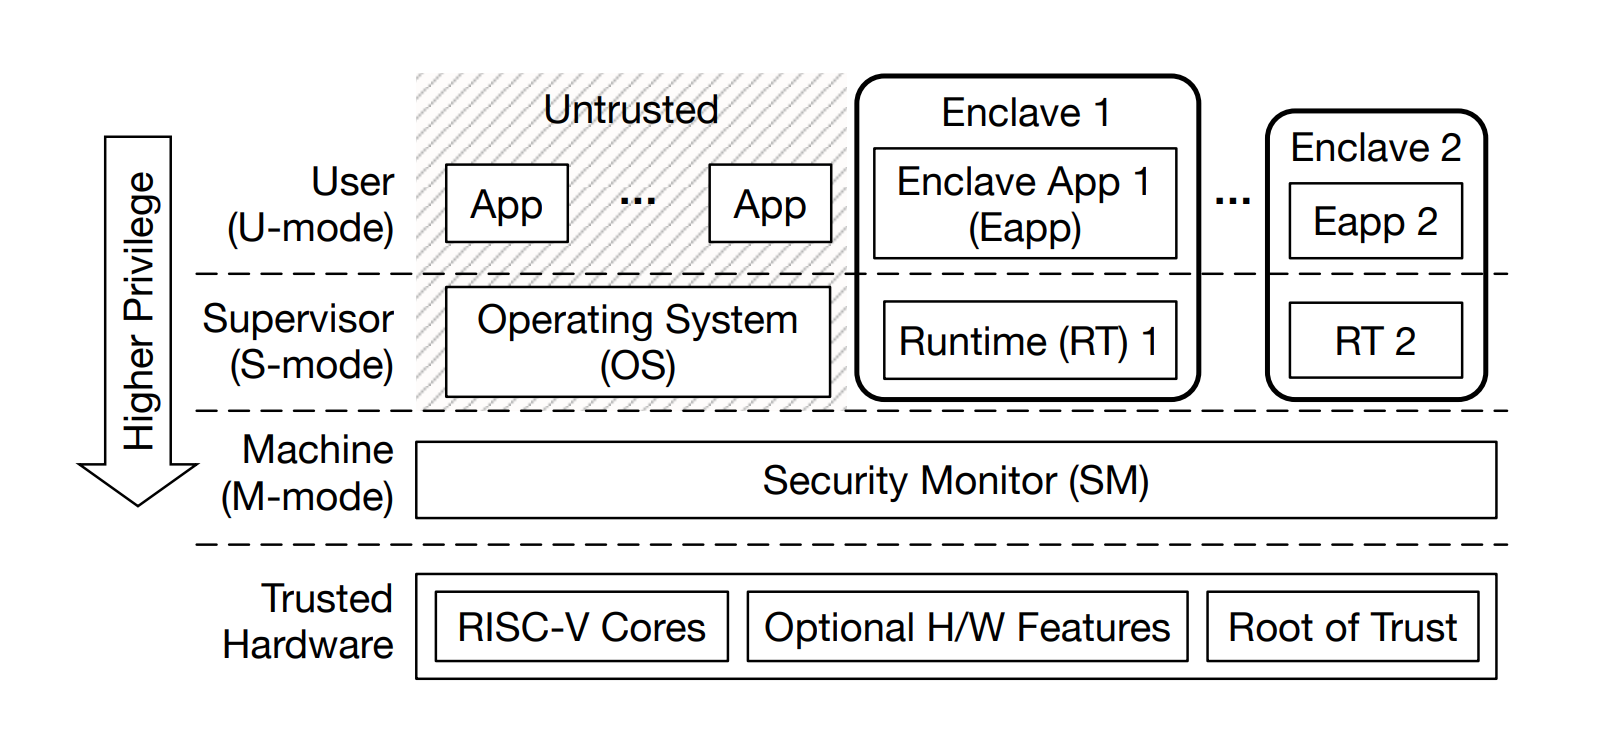
\includegraphics[scale=0.35]{./chapters/images/keystone-components.png}
    \caption{Keystone system with host processes, untrusted OS, security monitor, and multiple enclaves (each with runtime and eapp) \cite{lee2020keystone}.}
    \label{keystoneComponents}
\end{figure}
\subsection*{Trusted Hardware}
Trusted Hardware is a CPU package built by an honest manufacturer that must enclose standard RISC-V cores that are Keystone compatible and a root of trust. Optional features on the hardware could also include memory encryption, cache partitioning, a cryptographically safe source of randomness, etc. Platform-specific plug-ins are needed by the Security Monitor to support optional features.
\subsection{Security Monitor}
Security Monitor (SM) is a trusted software that runs in M-mode and works as the small trusted computing base (TCB) in the Keystone system. Before the security monitor can be considered trusted, first it must be verified by the hardware root of trust. After the root of trust measures the SM, it generates a keypair for remote attestation, signs the public key, and then continues booting. The SM manages the isolation boundary between the enclaves and the untrusted OS, therefore it implements the majority of Keystone's security guarantees.  It serves as an interface for managing the enclave's lifecycle and utilising platform-specific features. The OS and enclaves may call SM functions using the Supervisor Binary Interface (SBI). Specifically, the SM provides the following functionality:
\begin{itemize}
    \item \textit{memory isolation} using RISC-V PMP
    \item \textit{remote attestation} (signatures and measurement): the goal is to demonstrate to a remote client that the enclave contains the expected application, and is running on trusted hardware
    \item and other features, such as system PMP synchronization, enclave thread management and side-channel defences  
\end{itemize}

\subsection{Runtime}
Keystone developers implemented the Runtime (RT) with the goal of minimal and flexible TCB. It is an S-mode software. As a result, enclave applications can use modular system-level abstraction (e.g., virtual memory management). It provides kernel-like functionality, such as system calls, trap handling, virtual memory management and so on. Although the RT functions similarly to a kernel inside an enclave, most kernel functionalities are not necessary for the enclave application. To allow enclave developers to include only the necessary functionality and minimize the TCB, keystone developers created an example of RT called Eyrie. It enables reusability since it is compatible with multiple-user programs. And by adding RT modules, they expand RT functionality without changing user applications or without complicating the SM.

\begin{figure}[h!]
    \centering
    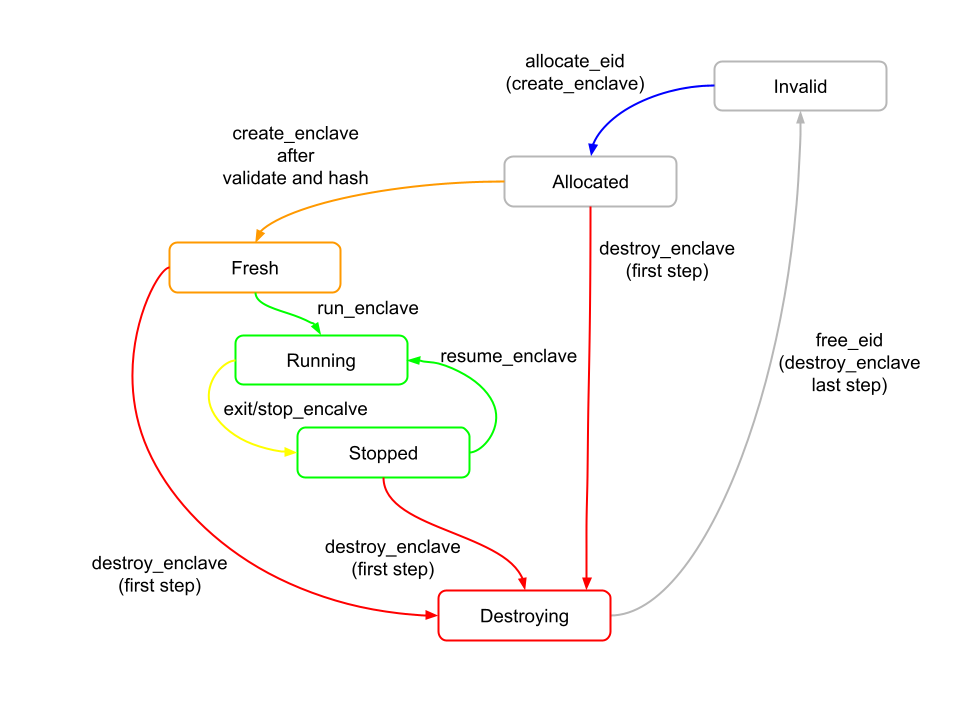
\includegraphics[scale=0.45]{./chapters/images/Enclave lifecycle.png}
    \caption{Enclave Lifecycle \cite{keystone-doc}.}
    \label{enclave-lifecycle}
\end{figure}

\subsection{Enclave}
An Enclave is an environment isolated from the untrusted OS and other enclaves. Each enclave is provided with a private physical memory region which is accessible by only the enclave and SM. Each enclave consists of a user-level enclave application called \textit{eapp} and a supervisor-level runtime. An eapp is a user-level application that executes in the enclave. A developer can create a custom eapp from scratch, or just execute an existing RISC-V binary in Keystone. The enclave lifecycle can be seen in figure \ref{enclave-lifecycle}. The main phases are:
\begin{itemize}
    \item \textit{creation}: when an enclave is started it has a contiguous range of physical memory that is called Enclave Private Memory (EPM). In the beginning, the EPM is allocated by the untrusted host, which initialises it with the enclave's page table, the runtime and the enclave application. When the untrusted host class the SM to create an enclave, the SM isolates and secures the EPM using a PMP entry, and then the PMP status is propagated throughout all of the system's cores. Subsequently, before the enclave execution, the enclave's initial state is measured and verified by the SM.
    \item \textit{execution}: the SM enters the enclave on one of the cores as soon as the untrusted asks for it. The PMP permission is enabled to the core by the SM, and the core starts running the eapp. The RT can exit or re-enter the enclave at any time. The PMP permissions are switched to keep the isolation each time a core exits or enters the enclave.
    \item \textit{destruction}: the untrusted host may want to destroy the enclave at any moment, when it happens, the EPM is cleared by the SM and the PMP entry is freed. The untrusted host then definitely reclaims the released memory.
\end{itemize}

\subsection{Edge Calls}
Function calls that enter or exit the enclave are known as \textit{edge calls} in Keystone, as in other enclave systems. For instance, if an enclave wants to send a network packet, it must use an edge call to deliver the data to an untrusted host process. The current version of Keystone allows \textit{enclave} $\rightarrow$ \textit{untrusted host} calls, also known internally as \textit{ocalls} (outbound calls, names under discussion). In the current version of Keystone, all ocall wrapping code uses shared memory regions to transfer data. When referencing data in these regions virtual address pointers are never used, instead, only offsets into the region are used \cite{keystone-doc}. \\
 
\begin{figure}[h!]
    \centering
    \includesvg[inkscapelatex=false, scale=0.55]{./chapters/images/ocall.svg}
    \caption{Simplified example of an ocall lifecycle \cite{keystone-doc}.}
    \label{ocall-lifecycle}
\end{figure}

\subsubsection{Edge Calls Lifecycle}
Consider for example a generic \texttt{ocall\_do\_something}. This call transfers some values passed as arguments from the enclave to be processed by the host process. (It could be a value to be printed, a file to be stored and so on). The enclave application calls \texttt{ocall\_do\_something(...)}, which is an edge wrapper function.
\texttt{ocall\_do\_something(...)} uses the system-call-like interface to the runtime to execute an \textit{ocalls} similar to \texttt{ocall(OCALL\_DO\_SOMETHING, \&input, sizeof(input), \&ouput,  sizeof(output))}. It passes a pointer to the value, the size of the argument, and any necessary return buffer information. 
After allocating an \texttt{edge\_call} structure in the shared memory region, the runtime fills out the call type, copies the value into another part of the shared memory, and sets up the offset to the argument value. Note that in Keystone edge calls employ offset values in the shared memory area, rather than pointers.
The runtime subsequently exits the enclave with an \texttt{SBI\_CALL}, i.e., \texttt{sbi\_stop\_enclave()}, passing a value indicating that the enclave is executing an \textit{ocalls} rather than shutting down. 
After checking the enclave's exit state and noting a pending \textit{ocalls}, the Keystone kernel driver resumes execution before handing control to the userspace host process. 
The registered \textit{ocalls} handler wrapper for \texttt{OCALL\_DO\_SOMETHING} is dispatched by the userspace host process, which also consumes the edge call. The wrapper generates a pointer to the argument value from the offset in the shared memory region and then calls \texttt{do\_something} with the value as an argument. The host wrapper determines whether any return values must be copied into the shared memory region upon return and returns the control to the driver after setting the edge call return status to \texttt{SUCCESS}. Through an \texttt{SBI\_CALL}, the driver rejoins the enclave runtime. The enclave \textit{ocalls} wrapper code is resumed once the runtime determines whether any return information has to be copied from the shared region into return buffers. Finally, the function that has called at the beginning \texttt{ocall\_do\_something} receives any return values from the \textit{ocalls} wrapper code \cite{keystone-doc}.


\section{Memory isolation using RISC-V PMP}
In Keystone, developers refer to the memory section that an enclave uses as a \textit{region} and each region is defined by a PMP entry. Currently, the SM employs two PMP registers for internal purposes (i.e., security monitor memory and untrusted memory). One active enclave may use one of the remaining PMP entries each. RISC-V PMP has several properties, the most relevant are: 
\begin{itemize}
    \item prioritization by index: the index of PMP entries statically determines the priority. Indices go from \texttt{0} to \texttt{N}, where \texttt{N} depends upon the platform. \texttt{0} is the highest priority,whereas \texttt{N} is the lowest. 
    \item default denies: if no PMP entry matches with an address, the memory access will be rejected by default.
\end{itemize}
For simplicity, in the following explanation PMP entries are denoted as \texttt{pmp[i]} where \texttt{i} is an index. At the start of the boot process, physical memory is not accessible by U- or S-modes. \\

\begin{lstlisting}[frame=single,showspaces=true,caption={Memory state when booting start \cite{keystone-doc}},captionpos=b,label={sm-pmp-1}]
-: inaccessible (NO_PERM), =: accessible (ALL_PERM)

pmp[1:N]    |                                       | : undefined
net result  |---------------------------------------|   
\end{lstlisting}
\noindent
The SM sets the highest priority PMP entry to cover the address range containing itself and sets all permission bits to 0. Suddenly, the SM sets the lowest priority PMP entry to cover the full memory and sets all permission bits to 1, this will allow the OS to access the remaining memory and start booting. The result can be seen below in listing \ref{sm-pmp-2}. \\

\begin{lstlisting}[frame=single,showspaces=true,caption={Memory state just after booting \cite{keystone-doc}},captionpos=b,label={sm-pmp-2}]
-: inaccessible (NO_PERM), =: accessible (ALL_PERM)

pmp[0]       |-------|                              | : SM memory
pmp[others]  |                                      | : undefined
pmp[N]       |======================================| : OS memory
net result   |-------|==============================|
\end{lstlisting}
\noindent
Each time the SM creates an enclave, it will select a PMP entry for the enclave to defend its memory from other U-/S-mode software. This can be seen below in listing \ref{sm-pmp-3}. \\
\begin{lstlisting}[frame=single,showspaces=true,caption={Memory accessible by the untrusted host \cite{keystone-doc}},captionpos=b,label={sm-pmp-3}]
-: inaccessible (NO_PERM), =: accessible (ALL_PERM)

pmp[0]       |-------|                              | : SM memory
pmp[1]       |              |---------|             | : enclave 
                                                        memory
pmp[others]  |                                      | : undefined
pmp[N]       |======================================| : OS memory
net result   |-------|======|---------|=============|
\end{lstlisting}
\noindent
When the SM enters the enclave and executes the eapp, it flips the permission bits of the enclave's PMP entry and the last PMP entry. Untrusted shared buffer is the term for the contiguous memory region that Keystone enables the OS to allocate in the OS memory space in order to use it as an enclave's communication buffer. This is shown below in listing \ref{sm-pmp-4}.
The SM just flips the permission bits back when it leaves the enclave. When an enclave is destroyed by the SM, the PMP entry is made available for usage by other enclaves. \\
\begin{lstlisting}[frame=single,showspaces=true,caption={Memory accessible by a running enclave \cite{keystone-doc}},captionpos=b,label={sm-pmp-4}]
-: inaccessible (NO_PERM), =: accessible (ALL_PERM)

pmp[0]       |-------|                              | : SM memory
pmp[1]       |              |=========|             | : enclave 
                                                        memory
pmp[others]  |                                      | : undefined
pmp[N]       |                                |==|  | : untrusted 
                                                        shared 
                                                        buffer
net result   |-------|------|=========|-------|==|--|
\end{lstlisting}


\section{Keystone key-hierarchy}
Figure \ref{keystone-key-hierarchy} shows the key hierarchy of Keystone. The root of the key hierarchy is the asymmetric processor key pair (\texttt{SK\_D} and  \texttt{PK\_D}). The asymmetric security monitor key pair (\texttt{SK\_SK} and \texttt{PK\_SM}) is derived from the measurement of the security monitor (\texttt{H\_SM}) and the private processor key (\texttt{SK\_D}) \cite{keystone-doc}.
As a result, the computed security monitor key pair is bound to the processor and to the identity of the security monitor itself.

\begin{figure}[h!]
    \centering
    \includesvg[inkscapelatex=false, scale=0.60]{./chapters/images/Keystone key hierarchy.svg}
    \caption{The key hierarchy of Keystone \cite{keystone-doc}.}
    \label{keystone-key-hierarchy}
\end{figure}
\subsection{Sealing-Key Derivation}
In figure \ref{keystone-key-hierarchy} is also visible how sealing-keys are derived. An enclave can generate a key for data encryption using the data-sealing capability, enabling it to store data in untrusted non-volatile memory outside the enclave. This key is tied to the identity of the processor, the security monitor, and the enclave. As a result, only the same enclave using the same processor and security monitor can generate the same key. Data can be encrypted using this key and stored in unsecured, non-volatile memory. After an enclave restart, it can generate the same key once more, retrieve the encrypted data from the untrusted storage, and then use the derived key to decrypt it \cite{keystone-doc}.
A sealing key is computed starting from three inputs:
\begin{itemize}
    \item the private security monitor key (\texttt{SK\_SM})
    \item the hash of the enclave (\texttt{H\_SM})
    \item a key identifier
\end{itemize}
The key identifier is an extra input for the key derivation function selectable by the enclave. A single enclave can generate several keys by giving the key identifier various values.




\chapter{Self-Sovereign Identity as a Service}
%!TEX encoding = IsoLatin
%!TEX main = ../../main.tex

\subsection{Architecture}
{\color{red} ToDo: spiegare provisioning iniziale e architettura finale}
\begin{figure}[!h]
    \centering
    \includesvg[inkscapelatex=false, scale=0.7]{./chapters/images/manufacturer.svg}
    \caption{Manufacturer provisions device with expected hashes, keys and signature of the public key}
    \label{manufacturer-provisioning}
\end{figure}

\begin{figure}[!h]
    \centering
    \includesvg[inkscapelatex=false, scale=0.7]{./chapters/images/Demo architecture3.svg}
    \caption{Demo architecture}
    \label{poc-architecture}
\end{figure}

\chapter{Conclusion and Future Work}
%!TEX encoding = IsoLatin
%!TEX main = ../../main.tex

In conclusion, the goal of this work was to allow IoT-constrained devices to establish a secure communication channel with the edge device and trusted SSI-related operations computation on-demand. The designed architecture enables to access higher computational performances and more flexible hardware and software requirements. In the future, this opens up new scenarios employing additional and more modern cryptographic primitives for privacy-preserving credentials, which are yet not implemented in the current solution. 
Another future research topic could be the integration of a TLS connection between an external client and the enclave and how securely terminate TLS within the enclave, considering that the untrusted host proxies enclave messages. 
Additionally, another enhancement of the edge device could be the monitoring of the untrusted host integrity with a TPM.
This is just an introductory work to enable and ease the adoption of the Self-Sovereign Identity as a Service paradigm.


\appendix
%This chapters describes how the solution has been implemented and how to use it. 
%to configure the environment used for testing the proposed solution.
\chapter{User Manual}
%!TEX encoding = IsoLatin
%!TEX main = ../../main.tex

\section{Constrained and edge device comparison}
This section describes how to install and execute the code used for testing the cryptographic capabilities of constrained and non-constrained devices.
\subsection{Test MbedTLS library}
Mbed TLS \cite{mbed-tls} is a C library and it was used for testing RSA and ECDSA cryptographic primitives. The version used is \texttt{mbedtls-3.1.0}, available from this repository: \url{https://github.com/Mbed-TLS/mbedtls}. 

\subsubsection{Test on non-constrained device}
First, MbedTLS needs to be installed on the chosen system. \\
\begin{lstlisting}[style=terminal,frame=single]
$ wget 
 https://github.com/Mbed-TLS/mbedtls/archive/refs/tags/v3.1.0.zip
$ unzip v3.1.0.zip
$ cd mbedtls-3.1.0/
$ sudo make install
\end{lstlisting}
Once the library has been installed, enter the Mbed TLS test directory and compile the program.  \\
\begin{lstlisting}[style=terminal,frame=single]
$ cd mbedtls-test
$ gcc -o test main.c mytest.c -lmbedtls -lmbedx509 -lmbedcrypto
\end{lstlisting}
Then tests can be launched and the results can be stored on a file with the following command. \\
\begin{lstlisting}[style=terminal,frame=single]
$ ./test > results.txt
\end{lstlisting}
The output should be similar to the following shown in Fig. \ref{l-mbedtls-1}. \\
\begin{figure}[H]
\begin{lstlisting}[frame=single]
Seeding the random number generator... ok

Test: ECDSA key gen
p256
0.000266988,
0.000238424,
...
Test: ECDSA sign-gen
p256 key gen time: 0.000260937
0.000004468,0.000309109,0.001057424, # (hash, sign, ver) times
0.000003286,0.000296264,0.001026635,
...

Test: RSA 2048 key gen
0.133808741,
0.087886941,
...

Test: RSA sign-ver
rsa2048 key gen time: 0.065950689
0.000003988,0.002522734,0.000039014 # (hash, sign, ver) times
0.000003206,0.001853610,0.000038684
...
\end{lstlisting}
\caption{Example of MbedTLS tests output on a non-constrained device. \label{l-mbedtls-1}}
\end{figure}
\subsubsection{Test on constrained device}
STM32CubeIDE \cite{cube-ide} has been used (version \texttt{1.9.0}) for developing and flashing the binaries onto the STM32L4+ board \cite{stm32-board-product}.

For simplicity, the complete project is provided and it just needs to be imported into STM32CubeIDE as an existing project. Click \texttt{File > Import > Existing projects into Workspace}, then select the archive file \texttt{mbedtlsv1-stm32.zip} from the file system, select the project \texttt{Test1} and click \texttt{Finish}. Then plug the board into a USB port and click \texttt{Project > Build Project}. The code will be compiled. When it is done (and 0 errors appear in the console panel at the bottom), click \texttt{Run}. 

The output on the board is very similar to the previous one, for debug messages the output of the \texttt{printf} function is redirected to one \texttt{UART} and it can be read with a terminal emulator that supports serial port, such as \texttt{Teraterm} or \texttt{Putty}, by reading the \texttt{COM} that correspond to the \texttt{STM32} debugger. 
The output should be similar to the following shown in Fig. \ref{l-mbedtls-2}. \\
\begin{figure}[H]
\begin{lstlisting}[frame=single]
Seeding the random number generator... ok
Test: ECDSA key gen, sign-gen
p256
318,
316,
...
key gen time: 319
5;357;1257 # (hash, sign, ver) times
5;361;1264
\end{lstlisting}
\caption{Example of MbedTLS tests output on a constrained device. \label{l-mbedtls-2}}
\end{figure}

%Since it is just a test and some of them take a long time, it is suggested to choose and execute one test at a time by manually comment/uncomment the code in the file \texttt{mytest.c}. 

% \begin{lstlisting}[language=C,frame=single]
% printf("Test: ECDSA key gen, sign-gen\n");
% printf("p256\n");
% test_ECDSA_keygen(MBEDTLS_ECP_DP_SECP256R1, &ctr_drbg, iterations);
% test_ECDSA(MBEDTLS_ECP_DP_SECP256R1, MBEDTLS_MD_SHA256, &ctr_drbg, iterations);
% \end{lstlisting}


\subsection{Test BBS\texttt{+} signatures scheme}
BBS\texttt{+} rust library was used for testing BBS\texttt{+} signatures that can be used to generate signature proofs of knowledge and selective disclosure zero-knowledge proofs. In these tests, only simple single-message signing and verification were tested.

Before starting, we need to install Rust. The installation of Rust is through a tool called Rustup, which is a Rust installer and version management tool. The way to install Rustup differs by platform, on Unix, run the next command in the shell. This downloads and runs \texttt{rustup-init.sh}, which in turn downloads and runs the correct version of the \texttt{rustup-init} executable for your platform. For other platforms check the Rust documentation \cite{rust-install}. \\
\begin{lstlisting}[style=terminal,frame=single]
$ curl https://sh.rustup.rs -sSf | sh
\end{lstlisting}
When Rustup is installed, it will also add the latest stable version of the Rust build tool and package manager, also known as Cargo. The following commands will install dependencies and build the project. \\
\begin{lstlisting}[style=terminal,frame=single]
$ cd bbs-test
$ cargo build
\end{lstlisting}
To launch the test and take executions times of BBS\texttt{+} signatures and verification, run:  \\
\begin{lstlisting}[style=terminal,frame=single]
$ cargo run
\end{lstlisting}
The output should be similar to the following shown in Fig. \ref{l-bbs}. \\
\begin{figure}[H]
\begin{lstlisting}[frame=single]
AVG Time elapsed in key generation() is: 25 ms
AVG Time elapsed in sign() is: 18 ms
AVG Time elapsed in ver() is: 102 ms
\end{lstlisting}
\caption{Example of BBS\texttt{+} tests output. \label{l-bbs}}
\end{figure}

\section{Proof of concept}

The proof of concept relies on the full Keystone SDK. The easiest way for building and try Keystone and the proof of concept is to use QEMU. QEMU is an open-source machine emulator, in this case, is used to emulate RISC-V architecture.
The proof of concept has been tested with \texttt{Ubuntu 18.04}. 
\subsection{Keystone installation and requirements}
The following dependencies must be installed before installing Keystone. \\
\begin{lstlisting}[style=terminal,frame=single]
$ sudo apt update
$ sudo apt install autoconf automake autotools-dev bc \
  bison build-essential curl expat libexpat1-dev flex gawk \ 
  gcc git gperf libgmp-dev libmpc-dev libmpfr-dev libtool \ 
  texinfo tmux patchutils zlib1g-dev wget bzip2 patch vim-common \
  lbzip2 python pkg-config libglib2.0-dev libpixman-1-dev \
  libssl-dev screen device-tree-compiler expect makeself \
  unzip cpio rsync cmake p7zip-full
\end{lstlisting}
Then check out the Keystone repository and install everything with the quick setup script, it will install the RISC-V toolchain and if \texttt{KEYSTONE\_SDK\_DIR} environment variable is not set, it will also install Keystone SDK. \\
\begin{lstlisting}[style=terminal,frame=single]
$ git clone https://github.com/keystone-enclave/keystone.git
$ cd keystone
$ ./fast-setup.sh
\end{lstlisting}
If everything goes right, the following message is shown: \\
\begin{lstlisting}[frame=single]
    RISC-V toolchain and Keystone SDK have been fully setup
\end{lstlisting}
After running \texttt{fast-setup.sh}, run the following command to temporarily set in the current shell relevant environment variables: \\
\begin{lstlisting}[style=terminal,frame=single]
$ source source.sh
\end{lstlisting}
Otherwise for permanently store the environment variables, if bash is used this command will add the lines in \texttt{source.sh} to the shell's startup file: \\
\begin{lstlisting}[style=terminal,frame=single]
$ cat source.sh >> $HOME/.bashrc
\end{lstlisting}
CMake \cite{cmake} is used as a build system. As \texttt{<build directory>} the name \texttt{build} has been chosen. Then all components can be built, beware that this will take a while. \\
\begin{lstlisting}[style=terminal,frame=single]
$ mkdir build
$ cd build
$ cmake ..
$ make
\end{lstlisting}
\begin{mybox}
\faExclamation\enspace It has been noted that under \texttt{Windows Subsystem for Linux (WSL)} the build of the image can fail. To solve this issue just modify the \texttt{PATH} to not include \texttt{/mnt/c/*} folders.
\end{mybox}

\subsection{Build the demo}
Extract the provided zip file that contains the demo of the proof of concept. The extracted folder should contain the developed code explained in this document. The \texttt{riscv-musl-toolchain} has been used for building the \texttt{server\_eapp}, which can be set with the \texttt{./setup\_musl.sh} script. Then, the \texttt{./quick-start.sh} will build the demo, the script will create two files: \texttt{demo-server.ke} and \texttt{trusted\_client.riscv}. \\
\begin{lstlisting}[style=terminal,frame=single]
$ cd keystone-demo-poc
$ source ./setup_musl.sh
$ SM_HASH=./include/sm_expected_hash.h ./quick-start.sh
\end{lstlisting}
Then once the demo is built, the binaries need to be copied into the Keystone build folder. \\

\begin{lstlisting}[style=terminal,frame=single]
$ cp ./build/demo-server.ke ./build/trusted_client.riscv ../keystone/build/overlay/root/
\end{lstlisting}
Now the QEMU image can be re-generated. \\

\begin{lstlisting}[style=terminal,frame=single]
$ cd keystone/build
$ make image
\end{lstlisting}

\subsection{Run QEMU}
The following script will run QEMU, and start executing from the emulated silicon root of trust. The root of trust then jumps to the SM, and the SM boots Linux. \\
\begin{lstlisting}[style=terminal,frame=single]
$ cd keystone/build
$ ./scripts/run-qemu.sh
\end{lstlisting}
The script will start ssh on a random forwarded localhost port, which allows multiple test runs on the same development machine. The script will print what port it has forwarded ssh to on start. For example, to start a new shell in another window the next command can be used, and it is useful to run the client and the server in two different terminal windows. \\
\begin{lstlisting}[style=terminal,frame=single]
$ ssh root@localhost -p <port number>
\end{lstlisting}
Login as \texttt{\color{RedOrange}root} with the password \texttt{\color{RedOrange}sifive}. You can exit QEMU by \texttt{\color{RedOrange}ctrl-a\ `+`\ x} or using  \texttt{\color{RedOrange}poweroff}  command.

\subsection{Run the demo}
Inside QEMU, run the following commands. The first one will load the Keystone kernel module and the second one will set up the loopback device. \\
\begin{lstlisting}[style=terminal,frame=single]
> insmod keystone-driver.ko 
> ifdown lo && ifup lo           
\end{lstlisting}
On the server side run: \\
\begin{lstlisting}[style=terminal,frame=single]
> ./demo-server.ke         
\end{lstlisting}
On the client side run: \\
\begin{lstlisting}[style=terminal,frame=single]
> ./trusted_client.riscv 127.0.0.1        
\end{lstlisting}
The client will connect to the enclave and perform the remote attestation. If the attestation is successful, the client can send back the session context. Then, if server checks go right, the communication can start and the client can request operation to the server. 

If the enclave server app will be modified, the expected hash values have to be regenerated, otherwise, it can be tested with an option that will ignore the validation of the attestation report (it will still print the status of the validation). \\

\begin{lstlisting}[style=terminal,frame=single]
> ./trusted_client.riscv 127.0.0.1 --ignore-valid        
\end{lstlisting}

\subsection{Expected output}
The output of the client and the server should be similar to the following Figs. \ref{l-demo-c} and \ref{l-demo-s}.
\begin{figure}[H]
\begin{lstlisting}[frame=single]
              === Security Monitor ===
Hash: e51749130b6036fe85b27409a4ea3e1c078fe4dcb76eb697e7e3cdc5ff
313144628a1ec10558cea5ad94641de7fb31fda759758115caf1144b2c49603f
42db3a
Pubkey: cd98f4a28a8523ba8ecd31175aa0e2330b2f46e7034545254660126a
9f3b8cb9
Signature: e738f4e708f73ffa4a0d3dc2199c9e0ac119bf14b32da33afe842
66803c9ae0766eb6d9f83e6d3b2511cbe8443996feb0bf8714f35c0c678aa593
90846a8d50a
              === Enclave Application ===
Hash: 11ff35526c90c469ca6878dc22494703c554db65406dcc9942417be2d9
010722843d1bda7115604f518fabd47ec3ba79cd89a560847bb5b810c314201e
2217d6
Signature: 58ca380c6b4476ed7b27143d92dec14fff2858ffef8ed6ef40156
515d36da50a220e494d936cafedd23558b8d16ce66c6d5f00bdb7ec973ee46ec
f7a48c6fa0d
Enclave Data: b07dfd3047fb5213b8af9b76594a06891c893001c6c4be448a
d8b13f7eb02a19b27d0263bfd9aa8941345f837788159897a8aea2ecb33da926
b8d4747328eaace08a34d55fcdc41e2938838da173900485e99bcc1fb9eb7b00
dac1e2fe5a5174
                -- Device pubkey --
0faad4ff01178583baa588966f7c1ff32564dd17d7dc2b46cb50a84a69270b4c
[TC] Attestation signature and enclave hash are valid
[TC] Session keys established

        Available services
1. generate keys
2. store verifiable credential
3. get verifiable presentation
 . everything else to quit 
Type the service to request:
> 1
\end{lstlisting}
\caption{Example of output at client side. \label{l-demo-c}}
\end{figure}
\newpage


\begin{figure}[H]
\begin{lstlisting}[frame=single]
Verifying archive integrity... All good.
Uncompressing Keystone Enclave Package
[EH] Got connection from remote client
[SE] NOT USING REAL RANDOMNESS: TEST ONLY
[SE] Stub certificate signature is valid
[SE] [C] Successfully generated session keys.
[EH] Got an encrypted message:
3e5d0575e8bccf73 eb5255dad244eee1 93fcae78f5ad0459 ...

[SE] Sealing key derivation successful!
generate_public_keys

EdDSA_keys_t:  [192]
07FAC4B1522F06D916C55D321BB839F23AEF95AA48E051E53DB2AF284D7845...

Ciphertext  [208]
AB35E2D0F9C3ADFDD10E448D4ABD7A42E00ED87CE569C4AC3809785CC9A028...

Sign  [272]
FA72997814FA1F16D111DA0189D0440F0F245EB606BACACD0566DEB0767D44...
[EH] Saving sealed data
[EH] Filename: /root/075CFECFC6617F ... 26A116B1611_keys_sign
Response payload:  [64]
8E120A739BA94B7E9AE2F590166682170570D7AFCB70026B513405E56E90C1...
\end{lstlisting}
\caption{Example of output at server side. \label{l-demo-s}}
\end{figure}

\subsection{Tools for updating enclave and sm hashes}
If the SM or the eapp will be modified, the expected hashes need to be modified to generate a valid report for the client. The next command will create the necessary files in the \texttt{include} directory. The demo must be recompiled and the QEMU image rebuilt before and after this command is executed. \\

\begin{lstlisting}[style=terminal,frame=single]
# build the demo
# copy the binaries and build qemu image
$ KEYSTONE_BUILD_DIR=<path/to/keystone/build path> ./scripts/get_attestation_modified.sh ./include
# build the demo
# copy the binaries and build qemu image
\end{lstlisting}

If the \texttt{sm\_expected\_hash.h} is not present in the \texttt{include} folder, can be generated for the first time following the instruction in the \texttt{README.md} file of the SM repository available at the following url: \url{https://github.com/keystone-enclave/sm.git}. 

\subsection{Tools for provisioning}

The file \texttt{provision} can be used to generate a new \texttt{test\_client\_key.h}, which will contain the root key pair, the client key pair and the signature of the client public key made by the system administrator with its secrey key. 

It could be modified to meet your purposes (for example to generate more client key pairs and signatures or to use a fixed root key).
The program uses \texttt{libsodium} to generate an Ed25519 key pair for the system administrator. Then will generate another Ed25519 key pair for the client and the public part will be signed with the system administrator key pair. The server will use the system administrator public key to authenticate that the client is part of the system administrator network.
 
Once \texttt{libsodium}  has been installed, compile \texttt{provision.c}, run it and redirect the output to a file with the name \texttt{test\_client\_key.h}. 
The file \texttt{test\_client\_key.h} is already present in the \texttt{include} folder, but it may be necessary to generate a new one and it can be done with the following commands. \\

\begin{lstlisting}[style=terminal,frame=single]
$ git clone https://github.com/jedisct1/libsodium.git
$ cd libsodium
$ git checkout 4917510626c55c1f199ef7383ae164cf96044aea
$ ./configure
$ make && make check
$ sudo make install
$ sudo ldconfig

$ cd keystone-demo/provisioning
$ gcc -o provision provision.c -lsodium

$ ./provision > ../include/test_client_key.h
\end{lstlisting}
\chapter{Developer Manual}
%!TEX encoding = IsoLatin
%!TEX main = ../../main.tex

\section{Constrained and edge device comparison}
\subsection{Test MbedTLS library}
\texttt{mytest.c} is the most relevant file for this subproject. It is equal for both non-constrained devices and the constrained device (STM32L4+ board \cite{stm32-board-product}). The only difference is the function used for measuring the elapsed time of a cryptographic primitive. The function \texttt{clock\_gettime()}, of the standard library \texttt{time.h}, is used on the non-constrained device, while on the STM32L4+ board is used the \texttt{HAL\_GetTick()}. Figure \ref{pseudo-algo} describes in a pseudo-language how to measure the elapsed time of a cryptographic primitive. 
Then, the available tests are described. \\
\begin{figure}[H]
\begin{lstlisting}[language=C,frame=single]
  start = clock_gettime( ) or HAL_GetTick()
  // mbedtls cryptographic primitive
  end = clock_gettime( ) or  HAL_GetTick()
  print ( end - start ) // in ms
\end{lstlisting}
\caption{Pseudo algorithm for measuring the elapsed time. \label{pseudo-algo}}
\end{figure}

\noindent
\texttt{int test\_RSA\_keygen(\dots)}\\
It generates \texttt{N} RSA key pair and prints the elapsed for each generation in a CSV format. \\
\textit{Input}:
\begin{itemize}[noitemsep,nolistsep]
  \item \texttt{int key\_size}, size of the generated key (possible values: \texttt{2048}, \texttt{3072} or \texttt{4096})
  \item \texttt{mbedtls\_ctr\_drbg\_context *ctr\_drbg}, reference to \texttt{CTR\_DRBG} context structure for random number generation
  \item \texttt{int iterations}, number of times that the test will be executed
\end{itemize}
\textit{Output}: Returns \texttt{1} if successful, or an \texttt{MBEDTLS\_ERR\_XXX\_XXX} error code


\noindent
\texttt{int test\_RSA(\dots)}\\
It generates an RSA key pair, computes the RSA signature of a random hashed message (of 1024 bytes) and verifies the generated signature. Then, it prints the elapsed for each signature and verification in a CSV format. (Everything is repeated \texttt{N} times). \\
\textit{Input}:
\begin{itemize}[noitemsep,nolistsep]
  \item \texttt{int key\_size}, size of the generated key (possible values: \texttt{2048}, \texttt{3072} or \texttt{4096})
  \item \texttt{int sha\_alg},
  \item \texttt{mbedtls\_ctr\_drbg\_context *ctr\_drbg}, reference to \texttt{CTR\_DRBG} context structure for random number generation
  \item \texttt{int iterations}, number of times that the test will be executed
\end{itemize}
\textit{Output}:  Returns \texttt{1} if successful, or an \texttt{MBEDTLS\_ERR\_XXX\_XXX} error code


\noindent
\texttt{int test\_ECDSA\_keygen(\dots)}\\
It generates \texttt{N} EDSA key pair and prints the elapsed for each generation in a CSV format. \\
\textit{Input}:
\begin{itemize}[noitemsep,nolistsep]
  \item \texttt{int ecparams}, the identifier of domain parameters (curve, subgroup and generator),(possible values: \texttt{MBEDTLS\_ECP\_DP\_SECP256R1}, \texttt{MBEDTLS\_ECP\_DP\_SECP384R1} or \texttt{MBEDTLS\_ECP\_DP\_SECP521R1})
  \item \texttt{int sha\_alg},
  \item \texttt{mbedtls\_ctr\_drbg\_context *ctr\_drbg}, reference to \texttt{CTR\_DRBG} context structure for random number generation
  \item \texttt{int iterations}, number of times that the test will be executed
\end{itemize}
\textit{Output}:  Returns \texttt{1} if successful, or an \texttt{MBEDTLS\_ERR\_XXX\_XXX} error code


\noindent
\texttt{int test\_ECDSA(\dots)}\\
It generates an ECDSA key pair, computes the ECDSA signature of a random hashed message (of 1024 bytes) and verifies the generated signature. Then, it prints the elapsed for each signature and verification in a CSV format. (Everything is repeated \texttt{N} times). \\ \\
\textit{Input}:
\begin{itemize}[noitemsep,nolistsep]
  \item \texttt{int ecparams}, the identifier of domain parameters (curve, subgroup and generator),(possible values: \texttt{MBEDTLS\_ECP\_DP\_SECP256R1}, \texttt{MBEDTLS\_ECP\_DP\_SECP384R1} or \texttt{MBEDTLS\_ECP\_DP\_SECP521R1})
  \item \texttt{int sha\_alg}, digest algorithm (possible values: \texttt{MBEDTLS\_MD\_SHA256}, \texttt{MBEDTLS\_MD\_SHA384} or \texttt{MBEDTLS\_MD\_SHA512})
  \item \texttt{mbedtls\_ctr\_drbg\_context *ctr\_drbg}, reference to \texttt{CTR\_DRBG} context structure for random number generation
  \item \texttt{int iterations}, number of times that the test will be executed
\end{itemize}
\textit{Output}:  Returns \texttt{1} if successful, or an \texttt{MBEDTLS\_ERR\_XXX\_XXX} error code

% ===========================================================================
% SUBSECTION
% ===========================================================================

\subsection{Test BBS\texttt{+} signatures scheme}
For this subproject, the most relevant files are:
\begin{itemize}
  \item \texttt{Cargo.toml} where dependencies are added, such as  
  \texttt{bbs} and \texttt{rand}. 
  \item \texttt{main.rs} where tests for BBS\texttt{+} key generation, signature and verification are defined. 
  \begin{itemize} 
    \item \texttt{fn key\_gen\_test(iterations: usize)}
    \item \texttt{fn simple\_sign\_ver\_test(iterations: usize)}
    % \item \texttt{fn pok\_sign\_ver\_test(iterations: usize)}
  \end{itemize}
\end{itemize}
And the code is very simple, it launches the test for key generation and the test for signature and verification, operations are executed \texttt{iterations} times and the average is displayed on the output video.  \\
\begin{lstlisting}[frame=single]
fn main() {
  let iterations: usize = 100;
  key_gen_test(iterations);
  simple_sign_ver_test(iterations);
}
\end{lstlisting}


% ===========================================================================
% SUBSECTION
% ===========================================================================

\section{Proof of concept}
\subsection{Guide to Keystone Components}
The Keystone repository consists of several sub-components such as gitmodules or directories. This is a brief overview of them. \\
\begin{lstlisting}[frame=single]
+ keystone/
|-- patches/
|  # required patches for submodules
|-- bootrom/
|  # Keystone bootROM for QEMU virt board, including trusted boot chain.
|-- buildroot/
|  # Linux buildroot. Builds a minimal working Linux image for our test platforms.
|-- docs/
|  # Contains read-the-docs formatted and hosted documentation, such as this article.
|-- riscv-gnu-toolchain/
|  # Unmodified toolchain for building riscv targets. Required to build all other components.
|-- linux-keystone-driver/
|  # A loadable kernel module for Keystone enclave.
|-- linux/
|  # Linux kernel
|-- sm/
|  # OpenSBI firmware + Keystone security monitor
|-- qemu/
|  # QEMU
+-- sdk/
    # Tools, libraries, and example apps for building enclaves on Keystone        
\end{lstlisting}

\subsection{Guide to Keystone Demo Proof of concept}
The designed solution has been developed starting from the officially \texttt{kestone-demo} repository available at this link: \url{https://github.com/keystone-enclave/keystone-demo}, commit \texttt{8c6c0565e44f3d0e00bc3e4a6e77fc84c9e6d343}. The demo uses test keys and is not safe for production use. \\
\begin{lstlisting}[frame=single]
  + keystone-demo-poc/
  |-- docs/
  |  # Contains read-the-docs formatted and hosted documentation, such as this article.
  |-- include/
  |  # Contains shared files between eapp and client
  |-- provisioning/
  |  # C program to generate new client and root key pairs
  |-- scripts/
  |  # Contains a script for performing the attestation of sm and eapp
  |-- server_eapp/
  |  # small enclave server that is capable of remote attestation, secure channel creation, and performing a simple word-counting computation securely
  |-- sodium_patches/
  |  # Contains patch for libsodium that will run in the server eapp
  +-- trusted_client/
     # simple remote client that connects to the host, validates the enclave report, constructs a secure channel, and then can send messages to the host for computation.       
  \end{lstlisting}

\subsection{Relevant files of the demo}
Below are explained relevant files that change from the official \texttt{kestone-demo} repository.

\subsubsection{include/eh\_shared.h}
This file is shared between the enclave and the untrusted host. It defines the following data structure for exchanging sealed (encrypted) data between the enclave and the untrusted host. \\

\begin{lstlisting}[language=C,frame=single]
typedef struct stored_data_t{
  unsigned short file_type;
  unsigned char client_pk[crypto_kx_PUBLICKEYBYTES];
  size_t c_len; // content len 
  unsigned char content[]; // Flexible member
} stored_data_t;    
\end{lstlisting}

\subsubsection{include/messages.h}
This file is shared between the client and the enclave and it defines the messages (request amd response) they exchange. \\
\begin{lstlisting}[language=C,frame=single]
typedef struct request_message_t {
  unsigned short request_type;
  unsigned char secret[SECRET_LEN];
  size_t len;
  unsigned char payload[]; // Flexible member
} request_message_t;

typedef struct response_message_t {
  unsigned short response_type;
  size_t len;
  unsigned char payload[]; // Flexible member
} response_message_t;
\end{lstlisting}

\subsubsection{include/session\_context.c and include/session\_context.h}
The session context is the structure that the client provides to the enclave to prove that is built by a trusted manufacturer. With the function \texttt{session\_context\_from\_buffer} the session context is extracted from the received buffer. \\
\begin{lstlisting}[language=C,frame=single]
struct session_context_t {
  unsigned char  dh_public_key[PUBLIC_KEY_SIZE];
  unsigned char  challenge[CHALLENGE_SIZE];
  unsigned char  data_signature[SIGNATURE_SIZE];
  
  unsigned char  client_public_key[PUBLIC_KEY_SIZE];
  unsigned char  root_signature_of_client_pk[SIGNATURE_SIZE];
};

void session_context_from_buffer(struct session_context_t* session_context, unsigned char* buffer);
\end{lstlisting}

\noindent
\texttt{int session\_context\_verify(\dots)}\\
\textit{Input}:
\begin{itemize}[noitemsep,nolistsep]
  \item \texttt{struct session\_context\_t session\_context}, the session context to verify
  \item \texttt{unsigned char* challange}, the challenge that the server has sent to the client
  \item \texttt{const unsigned char* root\_public\_key}, the public key of the manufacturer
\end{itemize}
\textit{Output}: an \texttt{int} value, 1 if it is a valid session context, 0 if not.

\subsubsection{server\_eapp/service.c and server\_eapp/service.h}
The file \texttt{service.h} just exposes the function that processes the request received by the client. \\   
\begin{lstlisting}[language=C,frame=single]
response_message_t* process_request(request_message_t *request, size_t *pt_finalsize) {

  setup_sealing_material(request->secret);

  switch (request->request_type) {
  case SERVICE_GEN_KEYS:
    return generate_public_keys(pt_finalsize, EdDSA);
    break;
  case SERVICE_STORE_VC:
    return store_verifiable_credential(pt_finalsize, request->payload, request->len);
    break;
  case SERVICE_GET_VP:
    return get_verifiable_presentation(pt_finalsize, request->payload, request->len, EdDSA);
    break;
  }
  return NULL;
}
\end{lstlisting}

\noindent
\texttt{void store\_data (\dots)}\\
It saves the sealed data in untrusted non-volatile memory. \\
\textit{Input}:
\begin{itemize}[noitemsep,nolistsep]
  \item \texttt{unsigned char* buffer}, data to save
  \item \texttt{size\_t len}, lenght of the data to save
  \item \texttt{unsigned short file\_type}, type of the data to save (possible values: \texttt{FILE\_CLI\-ENT\_KEYS\_SIGNATURE} or \texttt{FILE\_CLIENT\_VC\_SIGNATURE})
\end{itemize}
\textit{Output}: none

\noindent
\texttt{unsigned char* seal\_data\_and\_sign (\dots)}\\
It encrypts and signs the data to save in untrusted non-volatile memory. \\
\textit{Input}:
\begin{itemize}[noitemsep,nolistsep]
  \item \texttt{unsigned char* data}, data to encrypt and sign
  \item \texttt{size\_t data\_len}, length of the data to encrypt and sign
  \item \texttt{size\_t* sign\_len}, pointer to store the actual length of the signed message
\end{itemize}
\textit{Output}: the signed message, which includes the signature plus an unaltered copy of the message. 


\noindent
\texttt{response\_message\_t* build\_response (\dots)}\\
It builds the response to sand back to the client. \\
\textit{Input}:
\begin{itemize}[noitemsep,nolistsep]
\item \texttt{size\_t* pt\_finalsize}, pointer to store the final length of the response
\item \texttt{unsigned short response\_type}, type of the response (possible values: \texttt{SERVICE\_\-GEN\_KEYS}, \texttt{SERVICE\_STORE\_VC}, \texttt{SERVICE\_GET\_VP}, \texttt{MSG\_EXIT})
\item \texttt{unsigned char *buffer}, response to send back to the client
\item \texttt{size\_t len}, length of the response
\end{itemize}
\textit{Output}: the built response 


\noindent
\texttt{response\_message\_t* generate\_public\_keys (\dots)}\\
It handles the request of the client to generate two key pairs. It saves the key pairs sealed in the untrusted non-volatile memory and sends back to the client only the public part. \\ 
\textit{Input}:
\begin{itemize}[noitemsep,nolistsep]
\item \texttt{size\_t* pt\_finalsize}, pointer to store the final length of the response
\item \texttt{int key\_type}, the key type that the client chooses to generate (for demo purposes only \texttt{EdDSA} can be generated, in future \texttt{BBS+} signature scheme will be implemented)
\end{itemize}
\textit{Output}: the built response 

\noindent
\texttt{response\_message\_t* store\_verifiable\_credential (\dots)}\\
It handles the request of the client to store a verifiable credential that the client obtained from an issuer. It saves the verifiable credential sealed in the untrusted non-volatile memory and sends back to the client a \texttt{0} if everything goes right. \\
\textit{Input}:
\begin{itemize}[noitemsep,nolistsep]
  \item \texttt{size\_t* pt\_finalsize}, pointer to store the final length of the response
  \item \texttt{unsigned char* vc}, verifiable credential to be stored
  \item \texttt{size\_t vc\_len}, length of the verifiable credential to be stored
\end{itemize}
\textit{Output}: the built response 

\noindent
\texttt{response\_message\_t* get\_verifiable\_presentation (\dots)}\\
It handles the request of the client to generate a verifiable presentation to use when interacting with a verifier. It retrieves from the untrusted non-volatile memory the previously stored verifiable credential and key pairs and sends back to the client the sign of the verifiable credential with one using an assertion key of the type that the client chose. \\
\textit{Input}:
\begin{itemize}[noitemsep,nolistsep]
  \item \texttt{size\_t* pt\_finalsize}, pointer to store the final length of the response
  \item \texttt{unsigned char* nonce}, \textit{(optional)} nonce that the verifier asks the client to insert in the verifiable presentation  
  \item \texttt{size\_t nonce\_len}, length of nonce
  \item \texttt{int key\_type}, the key type that the client previously chose to generate (for demo purposes only \texttt{EdDSA} can be used, in future \texttt{BBS+} signature scheme will be implemented)
\end{itemize}
\textit{Output}: the built response 

\subsubsection{server\_eapp/server\_eapp.c}
In this file, the important functions to mention are:
\begin{itemize}
  %\item \texttt{void validate\_session\_context(void* buffer, unsigned char* challange)}
  \item \texttt{void attest\_and\_establish\_channel()}: in this function, the server once has sent its report to the client and it waits for the session context of the client. Once received, it validates the session context and established the channel with the client
  \item \texttt{void handle\_requests()}: in this function, the server will wait for client requests, will processes the request (and interacts with the enclave host for data sealing) and send back the response to the client 
\end{itemize}
 
\subsubsection{trusted\_client/trusted\_client.c and trusted\_client/trusted\_client.h}
In this file, the important functions to mention are:

\noindent
\texttt{void gen\_session\_context(\dots)}\\
It generates the client session context that will contain a data part and the signature of the client's public key made by the system administrator at the provisioning phase. The data part is composed of a key for the Diffie Hellam key exchange protocol and the challenge sent by the server, all the data part is signed by the client's public key. \\
\textit{Input}:
\begin{itemize}[noitemsep,nolistsep]
  \item \texttt{byte* buffer}, pointer to the buffer that will contain the session context
\end{itemize}
\textit{Output}: none


\noindent
\texttt{request\_message\_t* generate\_request\_message(\dots)}\\
It builds the request message to request a service to the server. \\
\textit{Input}:
\begin{itemize}[noitemsep,nolistsep]
  \item \texttt{char* buffer}, a buffer of the data to send to the server (it can contain the key type or the verifiable credential)
  \item \texttt{size\_t buffer\_len}, length of the data
  \item \texttt{size\_t* finalsize}, a pointer to store the final length of the request message
  \item \texttt{unsigned char* secret}, the secret that the server will use to generate the sealing key in the key derivation function
  \item \texttt{unsigned short request\_type}, the request type that the client has chosen to send to the server (possible values: \texttt{SERVICE\_GEN\_KEYS}, \texttt{SERVICE\_STORE\_VC} or \texttt{SERVICE\_GET\_VP})
\end{itemize}
\textit{Output}: the built request message


\noindent
\texttt{request\_message\_t* generate\_exit\_message(\dots)}\\
It builds the request message to close the connection with the server.
\textit{Input}:
\begin{itemize}[noitemsep,nolistsep]
  \item \texttt{size\_t* finalsize}, a pointer to store the final length of the request message
\end{itemize}
\textit{Output}: the built exit request message


% ===========================================================================
% SUBSECTION
% ===========================================================================

% \begin{lstlisting}[language=C,frame=single]
   
% \end{lstlisting}

% \noindent
% \texttt{}\\
% \textit{Input}:\setlist{nolistsep}
% \begin{itemize}[noitemsep]
%   \item 
% \end{itemize}
% \textit{Output}: 


% bibliografia scritta "a mano"
%% !TEX encoding = IsoLatin

% La bibliografia, da inserirsi solo se ci sono state citazioni.
% In questo caso ricordarsi che bisogna sempre elaborare due volte il file .TEX
% perch� la prima volta viene generata la bibliografia mentre la seconda volta viene inclusa

% NOTA: citare il DOI non � obbligatorio ma MOLTO desiderabile
% NOTE: inserting the DOI is not compulsory bur STRONGLY recommended whenever it exists

\begin{thebibliography}{9} % se ci sono meno di 10 citazioni
%\begin{thebibliography}{99} % se ci sono da 10 a 99 citazioni
%\begin{thebibliography}{999} % se ci sono da 100 a 999 citazioni

% esempio citazione articolo a congresso
% example: reference to a conference paper
\bibitem{psisec}
% autori - authors
I.Enrici, M.Ancilli, A.Lioy,
% titolo articolo - article title
``A psychological approach to information technology security'',
% nome del congresso - conference name
HSI-2010: 3rd Int. Conf. on Human System Interactions,
% luogo (stato) e data del congresso
% town (country) and date of the conference
Rzesz�w (Poland), May 13-15, 2010,
% pagine dell'articolo - article pages
pp.\ 459-466,
% DOI
\doi{10.1109/HSI.2010.5514528}

% esempio citazione articolo su rivista
% example: reference to a journal/magazine article
\bibitem{tpa}
% autori- authors
G.Cabiddu, E.Cesena, R.Sassu, D.Vernizzi, G.Ramunno, A.Lioy,
% titolo dell'articolo -  article title
``Trusted Platform Agent'',
% nome della rivista - name of the journal
IEEE Software,
% volume e numero della rivista (alcune riviste non ce l'hanno)
% volume and issue number (some journals don't have it)
Vol.\ 28, No.\ 2,
% mese e anno di pubblicazione della rivista
% month and year when paper appeared in the journal
March-April 2011,
% pagine dell'articolo  - article pages
pp.\ 35-41,
% DOI
\doi{10.1109/MS.2010.160}


% esempio citazione capitolo di un libro fatto come collezione di contributi da autori diversi
% example: reference to the chapter of a book which is a collection of chapters from different authors
\bibitem{tc}
A.Lioy, G.Ramunno, % autori del capitolo
``Trusted Computing'' % titolo del capitolo
nel libro % in the book
``Handbook of Information and Communication Security'' % titolo del libro
a cura di % edited by
P.Stavroulakis, M.Stamp, % nomi dei curatori
Springer, % nome editore
2010, % anno di pubblicazione
pp.\ 697-717, % pagine del capitolo
\doi{10.1007/978-3-642-04117-4_32}

% esempio citazione pagina web di un progetto
% example: reference to the web page pof a project
\bibitem{openssl}
% nome del progetto - name of the project
The OpenSSL project,
 % URI della pagina web - URI of the web page
\url{http://www.openssl.org/}

% esempio citazione RFC
% example: reference to a RFC
\bibitem{tls12}
T.Dierks, E.Rescorla,
``The Transport Layer Security (TLS) Protocol Version 1.2'',
\rfc{5246}, August 2008,
\doi{10.17487/RFC5246}

% esempio: citazione libro
% example: reference to a book
\bibitem{seceng}
Ross J. Anderson,
``Security engineering'',
Wiley, 2008,
ISBN: 978-0-470-06852-6

\end{thebibliography}


% se la bibliografia ? stata scritta (usando Bibtex) nel file biblio.bib allora commentare la riga precedente e scommentare le due righe seguenti
\bibliographystyle{other/torsec}
\bibliography{other/biblio}

\end{document}
